\documentclass[twoside]{article}

\usepackage{aistats2026}
% If your paper is accepted, change the options for the package
% aistats2026 as follows:
%
%\usepackage[accepted]{aistats2026}
%
% This option will print headings for the title of your paper and
% headings for the authors names, plus a copyright note at the end of
% the first column of the first page.

% We also include a `preprint' option for non-anonymous preprints. 
% Change the options for the package aistats2026 as follows:
%
%\usepackage[preprint]{aistats2026}
%
% This option will print headings for the title of your paper and
% headings for the authors names, but does not print the copyright and 
% venue note at the end of the first column of the first page.

% If you set papersize explicitly, activate the following three lines:
%\special{papersize = 8.5in, 11in}
%\setlength{\pdfpageheight}{11in}
%\setlength{\pdfpagewidth}{8.5in}

% If you use the natbib package, activate the following three lines:
%\usepackage[round]{natbib}
%\renewcommand{\bibname}{References}
%\renewcommand{\bibsection}{\subsubsection*{\bibname}}

% If you use BibTeX in apalike style, activate the following line:
%\bibliographystyle{apalike}

% Packages. The style file loads amsmath only, so \mathbb and \bm need amssymb and bm.
\usepackage{amssymb}
\usepackage{amsthm}
\usepackage{bm}
\usepackage{graphicx}
\usepackage{booktabs}
\usepackage{multirow}

\usepackage[disable]{todonotes}
% \usepackage[]{todonotes}
\newcommand{\wmk}[2][] {\todo[inline,backgroundcolor=green!20!white, #1]{(Wouter) #2}}
\newcommand{\claude}[2][] {\todo[inline,backgroundcolor=blue!20!white, #1]{(Claude) #2}}

% Notation, following the conventions in .claude/skills/latex-writing-style.
\newcommand\given[1][]{\,#1\vert\,}
\providecommand{\dif}{\mathrm{d}}
\providecommand{\Ex}[2]{\mathbb{E}_{#1}\!\left[#2\right]}
\providecommand{\Var}[2]{\mathbb{V}_{#1}\!\left[#2\right]}
\providecommand{\Cov}[2]{\mathbb{C}_{#1}\!\left[#2\right]}

% Parametric distributions: a calligraphic capital, plus an upright lowercase where one
% letter will not do. \mathcal is defined for uppercase letters only.
\providecommand{\Gig}{\mathcal{GIG}}  % generalised inverse Gaussian
\providecommand{\Sic}{\mathcal{S}\mathrm{i}}   % Sichel
\providecommand{\NBin}{\mathcal{NB}}  % negative binomial

\usepackage[round]{natbib}
\renewcommand{\bibname}{References}
\renewcommand{\bibsection}{\subsubsection*{\bibname}}
\bibliographystyle{apalike}

\theoremstyle{plain}
\newtheorem{proposition}{Proposition}
\newtheorem{corollary}{Corollary}
\newtheorem{lemma}{Lemma}

\theoremstyle{definition}
\newtheorem{assumption}{Assumption}

\theoremstyle{remark}
\newtheorem{remark}{Remark}

\begin{document}

% If your paper is accepted and the title of your paper is very long,
% the style will print as headings an error message. Use the following
% command to supply a shorter title of your paper so that it can be
% used as headings.
%
%\runningtitle{I use this title instead because the last one was very long}

% If your paper is accepted and the number of authors is large, the
% style will print as headings an error message. Use the following
% command to supply a shorter version of the author names so that
% they can be used as headings (for example, use only the surnames)
%
%\runningauthor{Surname 1, Surname 2, Surname 3, ...., Surname n}

\twocolumn[

\aistatstitle{Actively sensing overdispersed count data\\ with Sichel distributed predictions}

\aistatsauthor{Wouter M. Kouw}

\aistatsaddress{Eindhoven University of Technology} ]

\begin{abstract}
Instruments that count photons, stones or events return data whose variance exceeds its mean, and the experimenter usually controls how long to count for.
We give a conjugate model for that situation: a Poisson likelihood whose rate carries a generalised inverse Gaussian prior, under actions that scale the rate by a known exposure.
The posterior stays in the family, the predictive is the Sichel law, and the expected information gain of a candidate action is available in closed form as a difference of two quantities that each cost one univariate evaluation.
We prove that the posterior concentrates on the true rate, with a condition on accumulated exposure rather than on the number of measurements, and we identify the arrangements in which the closed forms may actually be evaluated, since their Bessel functions overflow double precision at orders a belief reaches after a handful of counts.
Fitted to three measured fields of rates, the third parameter is decisive on two physical counting fields and worth nothing on a linguistic one, and the fitted order of the mixing law says in advance which case one is in.
In allocation studies the acquisition matters only when the budget cannot cover the contexts; criteria that ignore the aleatoric term then fail badly, while the closed form matches the best available alternatives at an order of magnitude less cost per decision.
\end{abstract}

\section{INTRODUCTION}
\label{sec:intro}

A great many instruments work by counting.
A detector records photons over a dwell time, a plant recovers stones from a volume of gravel, a survey meter accumulates events at a location.
In each case the experimenter chooses how much of the process to observe before seeing what it returns, and the budget for that choice is finite: seconds of telescope time, cubic metres of gravel, hours in the field.
Deciding where to spend it is an active sensing problem \citep{kreucher2005sensor,yu2009active}, and the natural score for a candidate is the information it is expected to carry \citep{lindley1956measure,chaloner1995bayesian}.

Two things make counts awkward.
The first is that they are almost never as regular as a Poisson process: the variance exceeds the mean, often by orders of magnitude, because the underlying rate varies across the contexts being sensed.
The second is that the expected information gain of a candidate action is an expectation of a Kullback-Leibler divergence over a predictive distribution, and outside a conjugate family it has to be estimated by nested Monte Carlo, which is expensive and biased \citep{rainforth2018nesting,rainforth2024modern}.
Conjugate models avoid the second problem, and the conjugate model for counts is the gamma-Poisson pair, whose predictive is negative binomial.
That family has a free mean and a free variance, so overdispersion alone is no reason to leave it.
What it does not have is a third parameter: once its first two moments are fixed, its tail is determined.

This paper takes the generalised inverse Gaussian as the mixing law instead.
It is conjugate to a Poisson likelihood, an action that scales the rate by a known exposure preserves that conjugacy, and the resulting predictive is the Sichel law \citep{sichel1975distribution,stein1987parameter}.
The extra parameter buys exactly the freedom the gamma lacks, which the count-modelling literature has long identified as the reason to reach for the Sichel: data that are overdispersed, heavily skewed and inflated at zero at the same time.
The distribution has been used to value diamond deposits, model word frequencies and fit species abundances.
As far as we have found, it has not been used to decide which measurements to take.

Our contributions are as follows.
We set out the model and its two closed forms, the conjugate update and the Sichel predictive, and show that every dependence on the action passes through a single scalar, so scoring a grid of candidates costs one evaluation apiece (Sections~\ref{sec:model} and \ref{sec:inference}).
We prove posterior consistency from an exact two-sided bound on a ratio of Bessel functions, with the condition falling on accumulated exposure rather than on the number of measurements, which for an adaptive sensor is a restriction on the policy rather than a formality (Proposition~\ref{prop:consistency}).
We show that analytic tractability and numerical reliability are different properties here, and give the arrangements in which the closed forms survive evaluation (Remark~\ref{rem:conditioning}).
Finally we ask what the model and the acquisition are each worth.
Fitted to three measured fields of rates, the third parameter is decisive on the two on which counting is a physical process and worthless on the one on which it is not, and the fitted order of the mixing law identifies which case one is in before any sensing is designed (Section~\ref{sec:experiments_fields}).
In allocation studies on two problems, the choice of acquisition is worth nothing until the budget is too small to cover the contexts, and is worth a great deal after that (Sections~\ref{sec:experiments_bulk} and \ref{sec:experiments_photon}).
\claude{Contribution list is deliberately modest about the acquisition. Our criterion ties EPIG and D-optimality on accuracy in every setting we ran; what it wins on is cost. Worth deciding whether the title should follow the evidence and lead with the model rather than the sensing.}


\section{PROBLEM STATEMENT}
We consider the problem of learning in a count data model where the rate parameters are a function of an input parameter. Let $y \in \mathcal{Y} \subseteq \mathbb{N}$ be the observed count variable, $x \in \mathcal{X} \subseteq \mathbb{R}^{D}$ and $u \in \mathcal{U}$ be the input variable. The goal is to predict the count observations $y$ at a given context latent state $x$ after input $u$.

\section{MODEL SPECIFICATION}
\label{sec:model}

We assume the counts are Poisson distributed under a rate variable. Our likelihood is:
%
\begin{equation}
    p(y \given x, u, \theta) = \mathcal{P}\Big(y \given f(u) \lambda(x)\Big) \,,
    \label{eq:likelihood}
\end{equation}
%
where $\mathcal{P}$ refers to a Poisson distribution function, $\lambda(x) > 0$ is the unknown emission rate at context $x$, and $f: \mathcal{U} \to [0, \infty)$ is an exposure variable. Examples of exposures include the dwell time of a detector, the integration time of a spectrometer, the aperture of a telescope, or the known attenuation between a source and a sensor \citep{}.

\begin{assumption}[Multiplicative exposure]
    \label{as:exposure}
    The input acts on the rate through a known scalar $f(u)$, which does not depend on the parameter $\theta$.
\end{assumption}

Assumption~\ref{as:exposure} carries the analytic results below, and it is worth naming what it excludes.
An input rescales the rate of the context it addresses, so it decides how much is measured.
It cannot change which parameter is measured, and no input renders one rate observable through another.
Inputs of this kind set the size of an update rather than its direction.

The context set is taken to be finite, with $K$ elements, so that the parameter is the vector of rates $\theta = (\lambda_1, \dots, \lambda_K)$ and an input addresses one of them.
These rates are independent under the prior and the likelihood factorises across contexts, so the remainder of this section treats a single context and writes $\lambda$ for the rate being addressed.
\claude{A continuous context set couples the rates and breaks this factorisation. Flagged for the discussion.}

\subsection{Prior Over the Rate}
\label{sec:model_prior}

Write $\Gig$ for the generalised inverse Gaussian law,
%
\begin{equation}
    \begin{split}
        p(\lambda) &= \Gig(\lambda \given \alpha, a, b) \\
        &= \frac{(b/a)^{\alpha/2}}{2 K_{\alpha}(\sqrt{ab})} \lambda^{\alpha - 1} \exp\big( -(a/\lambda + b \lambda)/2 \big) \,,
    \end{split}
    \label{eq:gig}
\end{equation}
%
with order $\alpha \in \mathbb{R}$, scale parameters $a, b > 0$, and $K_{\alpha}$ the modified Bessel function of the second kind.

Its three parameters separate once $(a, b)$ is traded for a scale $\eta = \sqrt{a/b}$ and a concentration $\omega = \sqrt{ab}$, because the mean of \eqref{eq:gig} is then
%
\begin{equation}
    \Ex{p(\lambda)}{\lambda} = \eta \frac{K_{\alpha + 1}(\omega)}{K_{\alpha}(\omega)} \,.
    \label{eq:gig_mean}
\end{equation}
%
Requiring a particular mean fixes $\eta$ in closed form and leaves $\alpha$ and $\omega$ free, so the brightness of a context and the shape of the uncertainty about it are set independently.

The gamma law is a boundary of this family rather than a competitor to it.
As $\omega \to 0$ with $\alpha > 0$, \eqref{eq:gig} tends to a gamma law of shape $\alpha$ and rate $b/2$, and the marginal of \eqref{eq:likelihood} tends to a negative binomial, written $\NBin$.
The conjugate Poisson pair is therefore contained in the model, at one edge of a parameter the model is otherwise free to move.

\subsection{Predictive Dispersion}
\label{sec:model_dispersion}

Marginalising the rate out of \eqref{eq:likelihood} gives the Sichel law, written $\Sic$, whose mass function is a ratio of normalising constants of \eqref{eq:gig} and is deferred to Section~\ref{sec:inference}.
Its first two moments follow from the laws of total expectation and variance without it,
%
\begin{align}
    \Ex{p(y \given u)}{y} &= f(u) \Ex{p(\lambda)}{\lambda} \,, \label{eq:predictive_mean} \\
    \Var{p(y \given u)}{y} &= f(u) \Ex{p(\lambda)}{\lambda} + f(u)^{2} \Var{p(\lambda)}{\lambda} \,, \label{eq:predictive_variance}
\end{align}
%
so that their ratio, the Fano factor, is
%
\begin{equation}
    F(u) = 1 + f(u) \frac{\Var{p(\lambda)}{\lambda}}{\Ex{p(\lambda)}{\lambda}} \,.
    \label{eq:fano}
\end{equation}

Two properties of \eqref{eq:fano} matter for what follows.

The first is that the departure from equidispersion is a function of the input.
A Poisson process has $F = 1$ everywhere, whereas here the second term grows linearly in the exposure, so how overdispersed the observations are is itself something the sensor decides.
Long dwells do not merely return larger counts, they return relatively more variable ones.

The second concerns what the third parameter of \eqref{eq:gig} is for.
A negative binomial already has a free mean and a free variance, so overdispersion on its own is no reason to leave the conjugate Poisson pair, and we do not claim otherwise.
What \eqref{eq:gig} adds is a third parameter which, with the predictive mean and variance both held fixed, remains free to move mass between the centre of the distribution and its tail.
That is the regime in which the count-modelling literature reaches for the Sichel law: observations that are at once overdispersed, heavily skewed and inflated at zero, where a two-parameter law cannot match the tail and the mode together.
\claude{Quantified but not yet in an experiment folder: at matched predictive mean and variance the Sichel tail mass beyond $y=50$ differs from the moment-matched negative binomial by factors from 216 down to 0.7 across $\omega$, and the mass at zero by up to 1.6.}
% TODO: cite. Sweep done 2026-08-08, full record in notes/sichel-literature-2026-08.md.
% Add these to Zotero first; references.bib is not edited by hand.
%   Sichel (1975), On a Distribution Law for Word Frequencies, JASA 70(351a), 542-547.
%   Stein, Zucchini & Juritz (1987), Parameter Estimation for the Sichel Distribution and
%     Its Multivariate Extension, JASA 82(399), 938-944.
%   Rigby, Stasinopoulos & Akantziliotou (2008), A framework for modelling overdispersed
%     count data, including the Poisson-shifted generalized inverse Gaussian distribution,
%     CSDA 53(2), 381-393.
%   Willmot (1987), The Poisson-inverse Gaussian distribution as an alternative to the
%     negative binomial, Scand. Actuarial J. 1987(3-4).
%   Low, Ong et al. (2017), Generalized Sichel Distribution and Associated Inference,
%     JSTA 16(3).

\section{INFERENCE}
\label{sec:inference}

A sensor needs two things: what a count tells it about the rate, and what it should expect the next count to be before committing to an input.
Assumption~\ref{as:exposure} makes both available in closed form, by the conjugacy of the generalised inverse Gaussian with a Poisson likelihood \citep{diaconis1979conjugate}.
Neither is available in the arrangement in which it is most compactly written, which Remark~\ref{rem:conditioning} takes up.

\subsection{Parameter Updating}
\label{sec:inference_update}

\begin{proposition}[Conjugate update]
    \label{prop:update}
    Under \eqref{eq:likelihood} and \eqref{eq:gig}, a count $y$ observed at input $u$ yields
    %
    \begin{equation}
        p(\lambda \given y, u) = \Gig\big(\lambda \given \alpha + y, \, a, \, b + 2 f(u) \big) \,.
        \label{eq:posterior}
    \end{equation}
\end{proposition}

The derivation is one line.
Multiplying \eqref{eq:likelihood} by \eqref{eq:gig} and dropping every factor free of $\lambda$ leaves
%
\begin{equation}
    \lambda^{\alpha + y - 1} \exp\big( -(a/\lambda + (b + 2 f(u)) \lambda)/2 \big) \,,
    \label{eq:posterior_kernel}
\end{equation}
%
which is the kernel of \eqref{eq:gig} at the stated parameters.

The three parameters play distinct roles under \eqref{eq:posterior}.
The count is absorbed by the order, which is the only place the data enter.
The input is absorbed by the second scale parameter, and it enters additively, so the update is the same whether an exposure is delivered in one measurement or split across several.
A sensor cannot manufacture information by fragmenting its budget.

The first scale parameter $a$ is not revised at all, which is worth a sentence because it governs \eqref{eq:gig} near the origin.
A Poisson likelihood carries information about the rate only through $\lambda^{y} e^{-f(u) \lambda}$, and neither factor has the $1/\lambda$ form that $a$ multiplies.
Whatever weight the prior places on very small rates is therefore never revised by counting, which is a modelling commitment rather than a defect.

\begin{corollary}[Two sufficient statistics]
    \label{cor:sufficient}
    After a history $\mathcal{D}_t = \{(y_i, u_i)\}_{i = 1}^{t}$ at one context,
    %
    \begin{equation}
        p(\lambda \given \mathcal{D}_t) = \Gig\Big(\lambda \given \alpha + \textstyle\sum_{i} y_i, \, a, \, b + 2 \sum_{i} f(u_i) \Big) \,.
        \label{eq:posterior_history}
    \end{equation}
\end{corollary}

Two consequences matter for a sensor that has to plan.
The history enters only through an accumulated count and an accumulated exposure, so a belief is two numbers per context whatever the horizon, and the state a planner carries does not grow with the number of measurements taken.
Both statistics are sums, so the posterior does not depend on the order in which those measurements were made.

The second of those statistics is chosen by the sensor, which raises a question a passive model does not have to answer: whether a policy that decides its own exposures still learns the rate.
Write $F_t = \sum_{i \leq t} f(u_i)$ for the exposure a context has accumulated by step $t$, and let the inputs be adapted, so that $u_i$ may depend on everything observed before it.

\begin{proposition}[Posterior consistency]
    \label{prop:consistency}
    Fix a context with true rate $\lambda^{*} > 0$ and a prior \eqref{eq:gig} with $a, b > 0$ and $\alpha \in \mathbb{R}$.
    If the policy is such that $F_t \to \infty$ almost surely, then
    %
    \begin{equation}
        \Ex{p(\lambda \given \mathcal{D}_t)}{(\lambda - \lambda^{*})^{2}} \longrightarrow 0
        \label{eq:consistency}
    \end{equation}
    %
    almost surely, so the posterior concentrates at $\lambda^{*}$, and its variance is $O(1/F_t)$.
    If instead $F_t \to F_{\infty} < \infty$, the posterior converges almost surely to a non-degenerate law and consistency fails.
\end{proposition}

The proof is in Appendix~\ref{appx:consistency}.
Three features of it are worth stating here.

The condition is on accumulated exposure and not on the number of measurements, which for an active sensor is a restriction on the policy rather than a formality.
A policy whose exposures decay quickly enough to be summable stops learning at a finite spread, however many measurements it goes on to take, and the second half of Proposition~\ref{prop:consistency} says this is the only way to fail.
Between the two regimes the rate is governed by $F_t$ throughout: exposures $f(u_i) \propto 1/i$ do diverge, but only logarithmically, and the posterior variance is still of order $1/\log t$.

The parameter $a$, which Proposition~\ref{prop:update} leaves untouched by every observation, does not obstruct concentration.
It enters the proof only through the width of a bracket around the posterior mean, a width proportional to $a$ and inversely proportional to the accumulated count, which therefore vanishes as counts arrive.
An unrevised parameter is not a floor on the posterior spread, because the mass it governs sits near the origin and the posterior moves away from there.

The rate is the one a Poisson likelihood permits and no better.
The elementary bound of Appendix~\ref{appx:consistency} gives the order $1/F_t$; sharpening it identifies the constant as $\lambda^{*}$, so the posterior variance approaches $\lambda^{*}/F_t$, the inverse Fisher information of a Poisson observed at total exposure $F_t$.
The three parameters that buy the tail behaviour of Section~\ref{sec:model_dispersion} are therefore free asymptotically: they cost nothing in the rate at which the rate itself is learned.

\subsection{Posterior Prediction}
\label{sec:inference_predictive}

Because \eqref{eq:posterior} returns the family to itself, we write $(\alpha, a, b)$ for the parameters of the current belief, prior and posterior alike, and drop the history from the notation.

\begin{proposition}[Posterior predictive]
    \label{prop:predictive}
    Under the belief $\Gig(\lambda \given \alpha, a, b)$, the count returned by input $u$ has mass function
    %
    \begin{equation}
        p(y \given u, \mathcal{D}) = \frac{(f(u) \eta_u)^{y}}{y!} \Big( \frac{\eta_u}{\eta} \Big)^{\alpha} \frac{K_{\alpha + y}(\omega_u)}{K_{\alpha}(\omega)} \,,
        \label{eq:sichel}
    \end{equation}
    %
    where $\eta_u = \sqrt{a / (b + 2 f(u))}$ and $\omega_u = \sqrt{a (b + 2 f(u))}$ are the scale and concentration of the updated belief in the coordinates of \eqref{eq:gig_mean}.
\end{proposition}

Equation~\eqref{eq:sichel} is the Sichel law $\Sic$, introduced by \citet{sichel1975distribution} as a model for word frequencies and studied since as the Poisson mixture of a generalised inverse Gaussian rate \citep{stein1987parameter}.
It follows from Proposition~\ref{prop:update} without further integration: the marginal of a count is the ratio of the normalising constant of the posterior to that of the prior, times the factor of the Poisson mass that does not involve the rate.
Its mean and variance are \eqref{eq:predictive_mean} and \eqref{eq:predictive_variance} evaluated at the current belief.

Every dependence of \eqref{eq:sichel} on the input is carried by the scalar $f(u)$, through the pair $(\eta_u, \omega_u)$.
Scoring a grid of candidate inputs therefore costs one evaluation per candidate against a belief that is computed once, and nothing has to be re-solved as the candidate changes.

The support of \eqref{eq:sichel} is unbounded, so a functional of the predictive that is not a moment, the entropy in particular, has no closed form and is computed as a sum over the support truncated at a fixed tail tolerance.

\begin{remark}[A closed form is not an evaluation recipe]
    \label{rem:conditioning}
    Equation~\eqref{eq:sichel} must not be evaluated as written.
    The Bessel function $K_{\alpha + y}$ overflows double precision at moderate order, and by Corollary~\ref{cor:sufficient} the order a belief carries is $\alpha + \sum_i y_i$, which grows without bound as counts accumulate.
    In the survey of Section~\ref{sec:experiments_verification} a direct call overflows after four measurements.
    Every quantity is therefore accumulated in logarithms, and the run of orders that the support sum requires is obtained by one of two routes, neither of which is uniformly better.
    The recurrence
    %
    \begin{equation}
        K_{\nu + 1}(z) = K_{\nu - 1}(z) + (2 \nu / z) K_{\nu}(z)
        \label{eq:bessel_recurrence}
    \end{equation}
    %
    adds two positive quantities, so no cancellation occurs at any order, and over the first few dozen orders it is exact to the last digit.
    Its rounding nevertheless compounds along the run: against $30$-digit references it is out by $3 \times 10^{-12}$ after $10^{3}$ orders and by $3 \times 10^{-7}$ after $2 \times 10^{5}$, where the uniform asymptotic expansion in the order is still exact, being a fixed-cost evaluation at each order rather than an accumulation.
    Short runs take the recurrence and long runs the expansion.
    Which route is needed is itself a modelling matter, since the length of the support sum is set by the weight of the predictive tail, and it is the heavy-tailed regime of Section~\ref{sec:model_dispersion} that makes the run long.
    Analytic tractability and numerical reliability are different properties, and only the first is settled by Proposition~\ref{prop:predictive}.
\end{remark}

\section{EXPERIMENTS}
\label{sec:experiments}

\subsection{Verification on GIG-Poisson data}
\label{sec:experiments_verification}

\begin{figure*}[t]
    \centering
    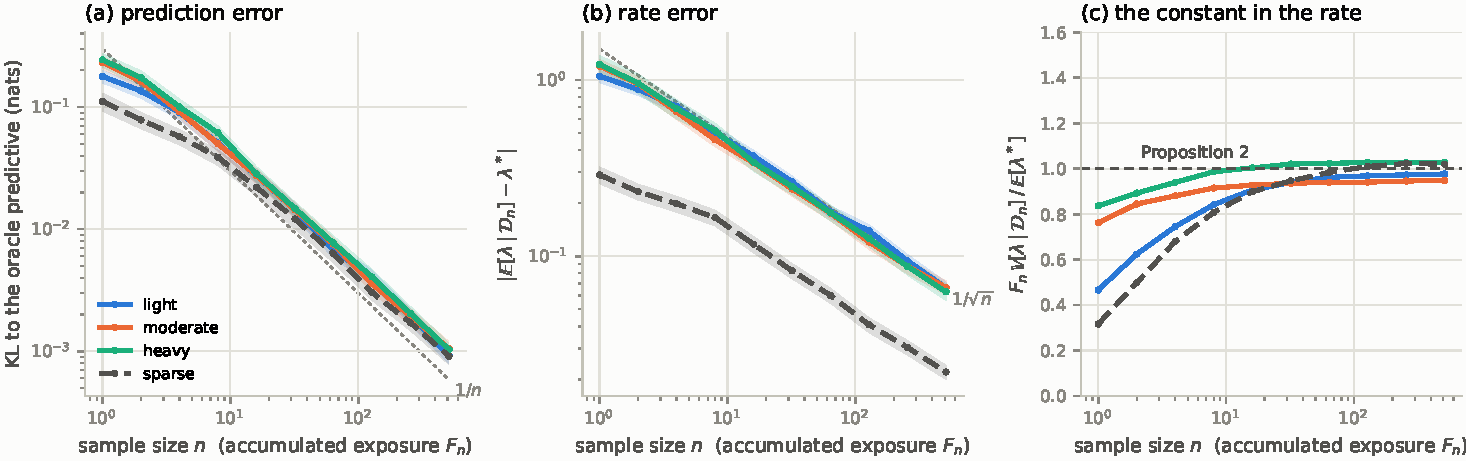
\includegraphics[width=\linewidth]{experiments/experiment-gigpoisson/figures/prediction}
    \caption{Prediction error against sample size on data the model specifies exactly, for four regimes of the generating parameters. Shaded bands are two standard errors over $400$ replicate rates. (a) Divergence from the oracle predictive falls as $1/n$. (b) The error in the posterior mean rate falls as $1/\sqrt{n}$. (c) The posterior variance rescaled by $F_n / \Ex{}{\lambda^{*}}$ collapses onto the constant predicted by Proposition~\ref{prop:consistency}, so the regime sets the constant only through the first few observations.}
    \label{fig:prediction}
\end{figure*}

\begin{table}[t]
    \caption{Fitted log-log slopes over the upper half of the sample-size range, by regime. The generating parameters change the constant, not the exponent.}
    \label{tab:prediction_slopes}
    \centering
    \begin{tabular}{lrrrr}
        \toprule
        regime & $\mathbb{V}/\mathbb{E}$ & KL & rate err. & $\mathbb{V}[\lambda \given \mathcal{D}_n]$ \\
        \midrule
        light & $0.8$ & $-0.971$ & $-0.492$ & $-0.987$ \\
        moderate & $4.0$ & $-0.952$ & $-0.472$ & $-0.995$ \\
        heavy & $40$ & $-0.959$ & $-0.498$ & $-0.997$ \\
        sparse & $0.5$ & $-0.935$ & $-0.480$ & $-0.973$ \\
        \midrule
        theory & & $-1$ & $-1/2$ & $-1$ \\
        \bottomrule
    \end{tabular}
\end{table}

Correct specification is arranged rather than assumed: rates are drawn from the mixing law \eqref{eq:gig} the sensor uses as its prior, and counts from the likelihood \eqref{eq:likelihood} it uses to update.
Any discrepancy is therefore attributable to the implementation.
Against $4 \times 10^{5}$ draws of the two-stage process, the predictive \eqref{eq:sichel} carries a support mass of one to $4 \times 10^{-13}$ and moments agreeing with a sum over the support to $9 \times 10^{-11}$; the conjugate update \eqref{eq:posterior} agrees with numerical Bayes to a total variation of $8 \times 10^{-13}$; and the largest log-ratio to the negative binomial obtained as $\omega \to 0$ falls as $\omega^{2}$.
Remark~\ref{rem:conditioning} is not hypothetical: evaluated in log space the Bessel quantities are accurate to $1.3 \times 10^{-13}$ against $40$-digit references, while a direct call to $K_{\nu}$ returns an infinity from order $97$, which a belief reaches after four measurements.

Figure~\ref{fig:prediction} and Table~\ref{tab:prediction_slopes} report how quickly the predictive approaches the one an oracle would use who knew the rate, over four regimes of the generating parameters and $400$ replicate rates each.
Prediction error falls as $n^{-1}$ and the rate error as $n^{-1/2}$ in every regime.
Panel (c) is the sharper test because it checks a constant: rescaling the posterior variance by $F_n / \Ex{}{\lambda^{*}}$ collapses all four regimes onto the value predicted by Proposition~\ref{prop:consistency} to within $2$ per cent, despite prior variance-to-mean ratios spanning a factor of $50$.
The generating parameters set the constant and not the exponent, and fifty times more prior dispersion costs roughly one extra observation.
\claude{Verification, not comparison: the competing models are not run here. A misspecified negative-binomial arm on the same data would be the natural addition.}

\subsection{Allocating a Bulk-Sampling Programme}
\label{sec:experiments_bulk}

\begin{figure*}[!t]
    \centering
    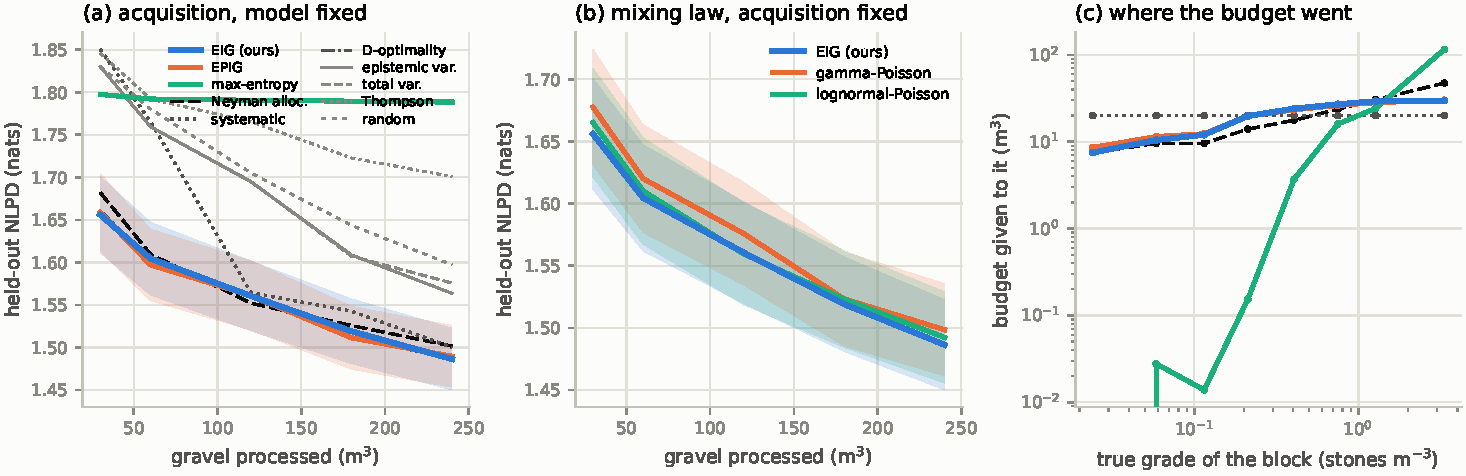
\includegraphics[width=\linewidth]{experiments/experiment-bulk-sampling/figures/bulk}
    \caption{Bulk sampling under a processing budget, 48 properties of 12 blocks each. Bands are one standard error. (a) Holding the model fixed and varying the acquisition. (b) Holding the acquisition fixed and varying the mixing law; note the axis, which spans a fifth of the range in (a). (c) Where the budget went, against what each block was worth: the systematic programme is flat by construction, the informed criteria tilt gently towards blocks with more to learn, and maximum entropy sampling abandons everything but the richest.}
    \label{fig:bulk}
\end{figure*}

\begin{table}[t]
    \caption{Bulk sampling at 12 blocks and 240 cubic metres, mean over 48 properties: held-out NLPD, grade RMSE, top-4 regret and milliseconds per decision. Superscripts are the paired $t$ against our agent, so negative favours ours and $|t| < 2$ is a tie. The upper block varies the acquisition with the model held fixed, the lower varies the mixing law with the acquisition held fixed. This is one point of the sweep in Figure~\ref{fig:scarcity}, and an abundant one.}
    \label{tab:bulk}
    \centering
    \footnotesize
    \setlength{\tabcolsep}{2pt}
    \begin{tabular}{lcccr}
        \toprule
        agent & NLPD & RMSE & regret & ms \\
        \midrule
        \multicolumn{5}{l}{\emph{acquisition, under the GIG-Poisson model}} \\
        EIG (ours) & $\mathbf{1.487}$ & $0.178$ & $0.016$ & $8.8$ \\
        EPIG & $1.490^{-1.4}$ & $0.179^{-0.2}$ & $0.016^{-0.1}$ & $74$ \\
        D-opt. & $1.488^{-0.4}$ & $0.187^{-2.0}$ & $0.018^{-0.4}$ & $0.5$ \\
        Neyman & $1.502^{-2.9}$ & $\mathbf{0.172}^{+0.7}$ & $0.016^{+0.0}$ & $1.0$ \\
        systematic & $1.500^{-3.3}$ & $0.221^{-5.4}$ & $\mathbf{0.015}^{+0.3}$ & $0.001$ \\
        epistemic & $1.564^{-7.0}$ & $0.229^{-3.1}$ & $0.032^{-2.1}$ & $1.6$ \\
        total var. & $1.576^{-6.2}$ & $0.261^{-2.4}$ & $0.038^{-2.4}$ & $1.6$ \\
        random & $1.597^{-8.3}$ & $0.482^{-4.4}$ & $0.046^{-3.2}$ & $0.01$ \\
        Thompson & $1.701^{-10.5}$ & $0.539^{-6.2}$ & $0.088^{-4.3}$ & $3.6$ \\
        max-ent. & $1.789^{-12.6}$ & $0.698^{-5.5}$ & $0.118^{-5.3}$ & $7.9$ \\
        \midrule
        \multicolumn{5}{l}{\emph{mixing law, under the EIG acquisition}} \\
        gamma-Poisson & $1.499^{-3.3}$ & $0.199^{-3.4}$ & $0.016^{-0.0}$ & $0.8$ \\
        lognormal-Pois. & $1.492^{-2.0}$ & $0.182^{-1.7}$ & $0.017^{-0.2}$ & $21$ \\
        \bottomrule
    \end{tabular}
\end{table}

The setting is the one the Sichel law was introduced for: diamonds occur in clusters, and it was the failure of the standard discrete laws to reproduce observed stone-count frequencies that motivated mixing a Poisson rate over a generalised inverse Gaussian \citep{sichel1975distribution,stein1987parameter}.
That model is used to value a deposit once samples are in hand, not to decide which samples to take.
A property is divided into $K$ blocks, block $k$ carries an unknown stone density $\lambda_k$, and an action is a pair $(k, v)$: which block to sample and how much gravel to process, from a schedule of $\{1, 2.5, 5, 10, 20, 40\}$ cubic metres.
The exposure is $f(u) = v r_k$ with $r_k$ the plant's known recovery factor, which is Assumption~\ref{as:exposure} exactly.

Two features of the design carry the comparison.
The budget is cubic metres of gravel rather than a number of samples, so every criterion is scored per cubic metre; counting in rounds would be won by whichever policy asks for the largest sample.
And the gravel is shared exactly: each block's stone field is realised once as a Poisson process in processed volume, so two policies that process the same gravel recover the same stones.
We report a held-out predictive score, the error in the estimated grade, and the grade forgone by committing to the four blocks a belief ranks highest.

Table~\ref{tab:bulk} reports both comparisons at twelve blocks and $240$ cubic metres.
Against every criterion that ignores the aleatoric term the result is decisive: maximum entropy sampling is the worst agent in the study, behind random, and panel (c) explains why.
Averaged over properties it touches $2.8$ of $12$ blocks, and on a representative property it puts $239$ of $240$ cubic metres into the single richest one.
The entropy of a count grows with its mean, so scoring a sample by how unpredictable its outcome is sends the budget to the block a sample tells one least about per unit of gravel, which is the aleatoric term of \eqref{eq:fano} acting as Section~\ref{sec:model_dispersion} describes.
Thompson sampling and both variance criteria fail the same way, spending on five or six blocks of twelve.

Against the criteria that use the same posterior as carefully, the accuracy is a tie: EPIG \citep{smith2023prediction} and D-optimality are indistinguishable from our agent on the predictive score, and no agent separates on the coarse ranking, which saturates once every block is visited.
On a model with one parameter per context, information about the rate and about the next count rank the candidates almost identically.
What separates them is cost: our acquisition is a closed form at $8.8$ milliseconds per decision where EPIG matches it at $74$, because its outer expectation needs a posterior predictive entropy at every node.
Holding the acquisition fixed instead, the third parameter is worth $0.012$ nats against the gamma boundary of its own family and $0.006$ against a lognormal.
Appendix~\ref{appx:grid} shows the two effects do not interact.

\begin{figure}[t]
    \centering
    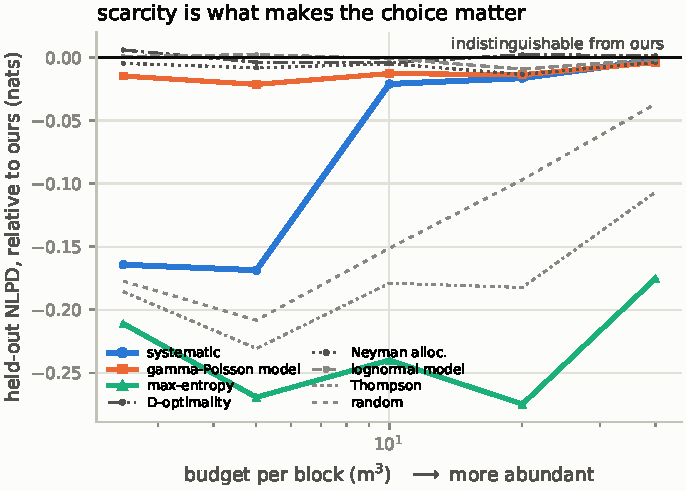
\includegraphics[width=\linewidth]{experiments/experiment-bulk-sampling/figures/scarcity}
    \caption{Predictive score relative to our agent as the budget per block is varied at fixed total budget, 24 properties per point. An agent on the zero line is indistinguishable from ours. The systematic programme sits on it while the budget is ample and leaves it once the budget cannot cover the blocks.}
    \label{fig:scarcity}
\end{figure}

Those numbers are one point on a curve.
Twelve blocks sharing $240$ cubic metres is enough that every block ends up well sampled whatever the schedule does, which is a poor place to compare schedules.
Figure~\ref{fig:scarcity} holds the budget fixed and varies the number of blocks it must cover.
The systematic programme is indistinguishable from our agent while the budget is ample, at $-0.002$ nats with forty cubic metres per block, and falls away once it is not, reaching $-0.169$ at $-8$ standard errors with five and $-0.164$ at $-14$ with two and a half.
The transition is sharp and sits between ten and five cubic metres per block, where a block stops being measurable in the share of the budget it can expect.
The choice of mixing law behaves the same way but an order of magnitude smaller, the gamma falling from $-0.004$ nats to between $-0.015$ and $-0.021$.
An adaptive schedule therefore earns its keep exactly when the budget cannot cover the contexts, and Section~\ref{sec:experiments_photon} is run at the scarce end for that reason.
\claude{This is a simulator whose structure is taken from the domain, not a field trial on a real deposit. Said plainly in the discussion; do not let the framing drift.}

\subsection{Scheduling a Gamma-Ray Observing Campaign}
\label{sec:experiments_photon}

\begin{figure*}[!t]
    \centering
    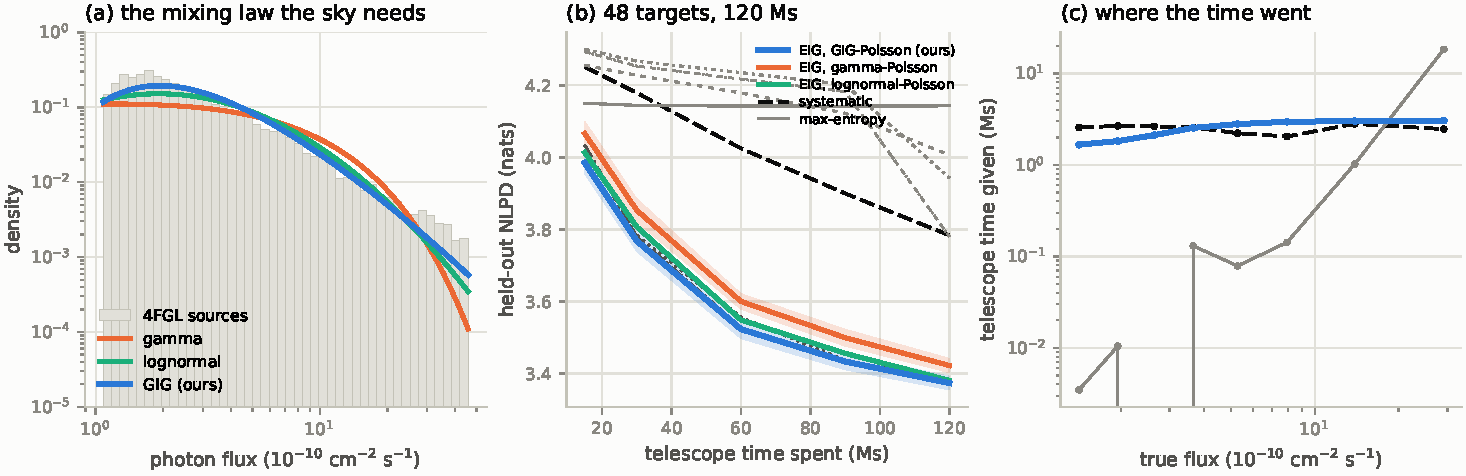
\includegraphics[width=\linewidth]{experiments/experiment-photon-counting/figures/photon}
    \caption{Scheduling telescope time across 48 gamma-ray targets on a budget of 120 megaseconds, 24 programmes. (a) The measured flux field of the Fermi-LAT catalogue against the maximum-likelihood fit of each mixing law. (b) Held-out predictive score against telescope time spent; bands are one standard error. (c) Time given to a target against how bright it turned out to be: maximum entropy sampling spends it all on the brightest, the informed criteria do not.}
    \label{fig:photon}
\end{figure*}

\begin{table}[t]
    \caption{Gamma-ray scheduling at the full budget, mean over 24 programmes. Superscripts are the paired $t$ against our agent; negative favours ours and $|t| < 2$ is a tie. The upper block varies the acquisition, the lower the mixing law.}
    \label{tab:photon}
    \centering
    \footnotesize
    \setlength{\tabcolsep}{2pt}
    \begin{tabular}{lcccr}
        \toprule
        agent & NLPD & dex & regret & ms \\
        \midrule
        \multicolumn{5}{l}{\emph{acquisition, under the GIG-Poisson model}} \\
        EIG (ours) & $3.373$ & $0.131$ & $0.0066$ & $16$ \\
        EPIG & $3.373^{+0.5}$ & $0.131^{+0.6}$ & $0.0066^{-0.4}$ & $127$ \\
        D-opt. & $3.373^{+0.2}$ & $0.130^{+0.5}$ & $0.0066^{+0.0}$ & $0.6$ \\
        Neyman & $3.380^{-0.6}$ & $0.139^{-3.8}$ & $0.0062^{+0.5}$ & $4.0$ \\
        systematic & $3.784^{-18.7}$ & $0.307^{-25.9}$ & $0.205^{-10.6}$ & $0.001$ \\
        total var. & $3.780^{-20.3}$ & $0.241^{-21.9}$ & $0.062^{-4.2}$ & $1.1$ \\
        Thompson & $3.943^{-32.1}$ & $0.317^{-33.8}$ & $0.158^{-7.1}$ & $15$ \\
        random & $4.006^{-23.2}$ & $0.344^{-29.0}$ & $0.270^{-8.2}$ & $0.01$ \\
        max-ent. & $4.143^{-32.5}$ & $0.389^{-40.8}$ & $0.276^{-8.2}$ & $13$ \\
        \midrule
        \multicolumn{5}{l}{\emph{mixing law, under the EIG acquisition}} \\
        gamma-Poisson & $3.422^{-7.4}$ & $0.145^{-4.7}$ & $0.0098^{-2.3}$ & $1.1$ \\
        lognormal-Pois. & $3.381^{-1.4}$ & $0.131^{-0.0}$ & $0.0063^{+0.3}$ & $146$ \\
        \bottomrule
    \end{tabular}
\end{table}

Every rate in the previous section is drawn from the law of Section~\ref{sec:model_prior}, so a model assuming that law is correct by construction.
Here the rates are the photon fluxes of $5065$ sources in the Fermi Large Area Telescope fourth source catalogue \citep{abdollahi2020fermi}, and the instrument that measured them is a photon counter, so the counting model of Section~\ref{sec:model_observation} is the measurement process rather than an analogy.
A pointed observation looks at one target at a time and the expected number of photons is the flux times the effective area times the time on target, so $f(u) = A_{\text{eff}} t$ and the budget is spent in megaseconds.
Priors are conditioned on the catalogue's source class, which an observer knows before pointing and which matters: pulsars have a median flux twelve times that of blazar candidates and a variance-to-mean ratio twelve hundred times larger.
The catalogue is split within each class, so priors are fitted to one half and sources drawn from the other.

Forty-eight targets share $120$ megaseconds, so most cannot be observed at all.
Under the same acquisition, the gamma mixing law is $0.049$ nats behind ours at $-7.4$ standard errors, $0.014$ dex behind on the flux estimate, and behind on the scheduling decision as well, which is the first setting here where the choice of model reaches the decision.
The lognormal ties us to within a standard error at nine times the cost per decision, so what the third parameter does not buy against that alternative the conjugacy buys instead.
The acquisition separates in the same regime: a systematic schedule is $0.41$ nats behind at $-18.7$ standard errors and maximum entropy sampling $0.77$ behind, while EPIG and D-optimality remain indistinguishable from our criterion, as they are in every setting we have run.

\subsection{Which Mixing Law Do Real Rate Fields Need?}
\label{sec:experiments_fields}

\begin{figure*}[!t]
    \centering
    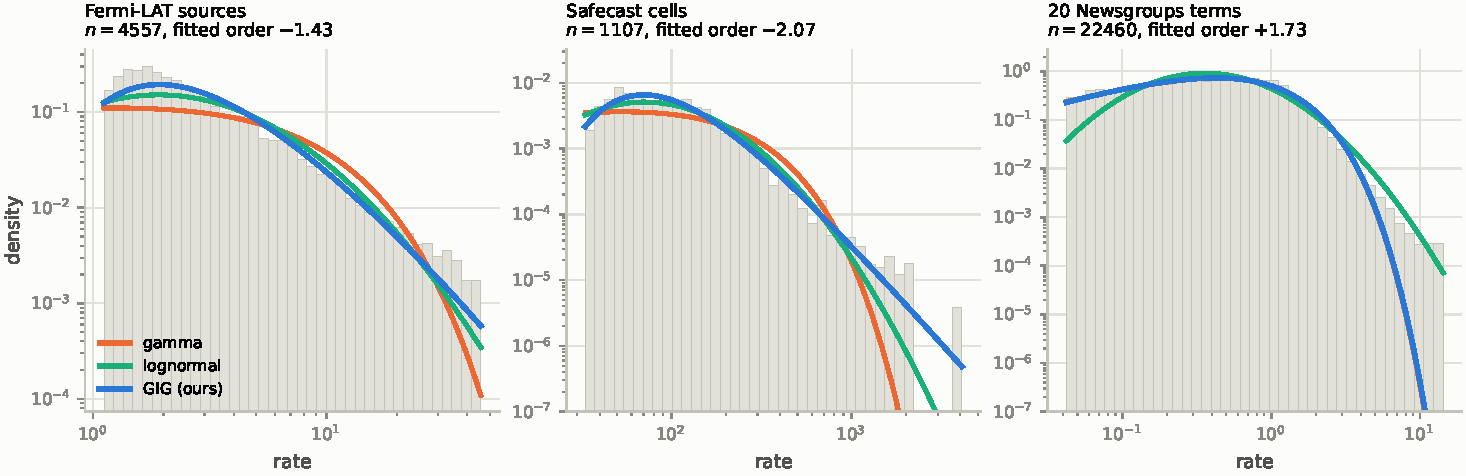
\includegraphics[width=\linewidth]{experiments/experiment-rate-fields/figures/rate_fields}
    \caption{Three measured fields of rates against the maximum-likelihood fit of each candidate mixing law. The fitted order is printed on each panel: the gamma occupies the edge of the family at a positive order, so a field whose order is fitted negative is one the gamma cannot reach however its two parameters are set. On the third panel the fitted order is positive and the gamma and the generalised inverse Gaussian coincide.}
    \label{fig:rate_fields}
\end{figure*}

\begin{table}[t]
    \caption{Three measured rate fields. $\Delta$AIC is against the best law for that field, so zero marks the winner. The last column is the advantage of the third parameter over the gamma per observation, which is the comparable figure across fields of different size.}
    \label{tab:rate_fields}
    \centering
    \footnotesize
    \setlength{\tabcolsep}{3pt}
    \begin{tabular}{llrrrr}
        \toprule
        field & law & $n$ & $\Delta$AIC & order & per obs. \\
        \midrule
        \multirow{3}{*}{Fermi-LAT} & gamma & & $1773$ & & \\
        & lognormal & $4557$ & $555$ & & $0.39$ \\
        & GIG & & $\mathbf{0}$ & $-1.43$ & \\
        \midrule
        \multirow{3}{*}{Safecast} & gamma & & $568$ & & \\
        & lognormal & $1107$ & $136$ & & $0.51$ \\
        & GIG & & $\mathbf{0}$ & $-2.07$ & \\
        \midrule
        \multirow{3}{*}{Newsgroups} & gamma & & $7$ & & \\
        & lognormal & $22460$ & $1362$ & & $0.00$ \\
        & GIG & & $\mathbf{0}$ & $+1.73$ & \\
        \bottomrule
    \end{tabular}
\end{table}

The comparisons above either generate their rates from \eqref{eq:gig} or argue from a single field.
This section asks three measured fields at once and allows them to disagree: the photon fluxes of Section~\ref{sec:experiments_photon}; the count rates of $1107$ five-hundred-metre cells around Fukushima Daiichi, recorded as counts per minute by the Geiger counters of the Safecast project \citep{brown2016safecast}; and, as a deliberate outsider, the relative rates of $1123$ terms across the twenty corpora of the 20 Newsgroups collection.
Each mixing law is fitted by maximum likelihood with the location held at zero and scored by AIC, so the third parameter pays for itself.
No acquisition, budget or policy enters.

On the two physical fields the third parameter is decisive, by $1773$ and $568$ points of AIC against the gamma; on the linguistic field it is worth $7$ points on $22460$ observations.
The fitted order says why.
A gamma is the boundary of the family at $\omega \to 0$ with a positive order, so a field whose order is fitted at $-1.43$ or $-2.07$ is one no gamma can reach however its two parameters are set, whereas one fitted at $+1.73$ sits inside the gamma's own range and the extra parameter has nothing left to do.
The question therefore has an answer that can be checked from the rates alone, before any sensing is designed, at the cost of one maximum-likelihood fit.
The ordering of the two-parameter laws is not stable across the three fields, so a practitioner who has settled on one of them has settled on the wrong one somewhere.
\claude{Two citations still missing from \texttt{references.bib}: Abdollahi et al. (2020), \emph{Fermi LAT Fourth Source Catalog}, ApJS 247, 33; and Brown et al. (2016), \emph{Safecast}, J.\ Radiol.\ Prot.\ 36(2), S82.}
\claude{Caveats were cut from this section on request as premature. They survive in each experiment's README: Fermi is flux-limited with estimated fluxes; Safecast is crowd-sourced from vehicles over years of decay, so a cell's rate is a mean over passes; and the Newsgroups field excludes terms absent from any group, which removes exactly the rare terms where burstiness is strongest. The last of these cuts against the result rather than for it, so it should return before the claim travels.}

\section{DISCUSSION}
\label{sec:discussion}

\paragraph{What the exposure assumption excludes.}
Assumption~\ref{as:exposure} asks that the action scale the rate by a known factor.
That covers a dwell time, an integration time, a processed volume and a known attenuation, and it is what keeps the family closed under observation.
It excludes an additive term.
A real gamma-ray observation counts source photons together with a known diffuse background, and a real survey meter counts contamination together with a natural background, so the rate is $f(u)\lambda + b$ rather than $f(u)\lambda$.
The mixture is no longer conjugate and the predictive is no longer Sichel.
This is the most concrete boundary of the framework we have found, and the obvious next question.

\paragraph{What the acquisition is and is not worth.}
Two criteria matched ours on accuracy in every setting we ran: the prediction-oriented EPIG \citep{smith2023prediction} and local D-optimality \citep{chaloner1995bayesian}.
We take that at face value.
On a model carrying one parameter per context, whose predictive depends on the belief only through that parameter, information about the rate and information about the next observation order the candidates almost identically, and the distinction that motivates a prediction-oriented acquisition does not arise.
What separates the three is cost: our criterion is a closed form, D-optimality is a moment, and EPIG requires an expectation over the candidate's own predictive with a posterior predictive entropy at every node.
The case for the work is therefore that a conjugate model makes a good acquisition cheap, not that it makes a better one.

The criteria that did separate, and badly, are those that ignore the aleatoric term.
Maximum entropy sampling \citep{sebastiani2000maximum} was the worst policy in both allocation studies, behind uniform random sampling.
The reason is visible in \eqref{eq:fano}: the entropy of a count grows with its mean, so a criterion that scores an action by how unpredictable its outcome is spends the budget where the noise is largest rather than where the uncertainty is.
That failure is a property of the criterion rather than of our family, since it reproduces under every mixing law we tried.

\paragraph{Scarcity is the operative variable.}
The single most consequential thing we found is not about any criterion.
When the budget is large enough that every context ends up well measured, no allocation rule can distinguish itself from visiting each in turn, and the prior differences that an adaptive rule would exploit are washed out by data.
The transition is sharp.
A study that reports one budget is reporting one point on that curve, and we would encourage the practice of sweeping it.

\paragraph{Limits of what we have shown.}
The two allocation studies are simulators whose structure is taken from their domains, not field trials, and only the rate fields of Section~\ref{sec:experiments_fields} are measured.
Contexts are treated as independent, which is what makes the belief factorise and the per-candidate cost a single evaluation; a spatial problem in which neighbouring cells inform each other would break that and is the extension we would attempt first.
And the rate of a context is taken to be fixed and unknown, so the overdispersion the model carries is uncertainty about it.
A process in which the rate is redrawn at every observation is a different model, and which of the two a given application needs is a question we have not settled.
\claude{That last point is unresolved and load-bearing: it decides what the right baselines are. See the memory note \texttt{overdispersion-has-two-readings}.}

\section{CONCLUSION}
\label{sec:conclusion}

Counting instruments with a controllable exposure admit a conjugate model richer than the gamma-Poisson pair.
Mixing a Poisson rate over a generalised inverse Gaussian keeps the posterior in the family, gives the Sichel law as the predictive, and puts the expected information gain of a candidate action in closed form, at an order of magnitude less cost per decision than the alternatives that match its accuracy.
The posterior concentrates on the true rate provided the policy lets accumulated exposure diverge, which for an adaptive sensor is a condition worth checking.
Whether the third parameter is worth its cost is a question about the field being sensed, and it can be answered from the rates alone before any sensing is designed: on the two physical counting fields we examined the fitted order of the mixing law lies outside the gamma's range, and on a linguistic one it does not.

\bibliography{references}

%%%%%%%%%%%%%%%%%%%%%%%%%%%%%%%%%%%%%%%%%%%%%%%%%%%%%%%%%%%%
\clearpage
\newpage
\section*{Checklist}


% %%% BEGIN INSTRUCTIONS %%%
The checklist follows the references. For each question, choose your answer from the three possible options: Yes, No, Not Applicable.  You are encouraged to include a justification to your answer, either by referencing the appropriate section of your paper or providing a brief inline description (1-2 sentences). 
Please do not modify the questions.  Note that the Checklist section does not count towards the page limit. Not including the checklist in the first submission won't result in desk rejection, although in such case we will ask you to upload it during the author response period and include it in camera ready (if accepted).

\textbf{In your paper, please delete this instructions block and only keep the Checklist section heading above along with the questions/answers below.}
% %%% END INSTRUCTIONS %%%


\begin{enumerate}

  \item For all models and algorithms presented, check if you include:
  \begin{enumerate}
    \item A clear description of the mathematical setting, assumptions, algorithm, and/or model. [Yes/No/Not Applicable]
    \item An analysis of the properties and complexity (time, space, sample size) of any algorithm. [Yes/No/Not Applicable]
    \item (Optional) Anonymized source code, with specification of all dependencies, including external libraries. [Yes/No/Not Applicable]
  \end{enumerate}

  \item For any theoretical claim, check if you include:
  \begin{enumerate}
    \item Statements of the full set of assumptions of all theoretical results. [Yes/No/Not Applicable]
    \item Complete proofs of all theoretical results. [Yes/No/Not Applicable]
    \item Clear explanations of any assumptions. [Yes/No/Not Applicable]     
  \end{enumerate}

  \item For all figures and tables that present empirical results, check if you include:
  \begin{enumerate}
    \item The code, data, and instructions needed to reproduce the main experimental results (either in the supplemental material or as a URL). [Yes/No/Not Applicable]
    \item All the training details (e.g., data splits, hyperparameters, how they were chosen). [Yes/No/Not Applicable]
    \item A clear definition of the specific measure or statistics and error bars (e.g., with respect to the random seed after running experiments multiple times). [Yes/No/Not Applicable]
    \item A description of the computing infrastructure used. (e.g., type of GPUs, internal cluster, or cloud provider). [Yes/No/Not Applicable]
  \end{enumerate}

  \item If you are using existing assets (e.g., code, data, models) or curating/releasing new assets, check if you include:
  \begin{enumerate}
    \item Citations of the creator If your work uses existing assets. [Yes/No/Not Applicable]
    \item The license information of the assets, if applicable. [Yes/No/Not Applicable]
    \item New assets either in the supplemental material or as a URL, if applicable. [Yes/No/Not Applicable]
    \item Information about consent from data providers/curators. [Yes/No/Not Applicable]
    \item Discussion of sensible content if applicable, e.g., personally identifiable information or offensive content. [Yes/No/Not Applicable]
  \end{enumerate}

  \item If you used crowdsourcing or conducted research with human subjects, check if you include:
  \begin{enumerate}
    \item The full text of instructions given to participants and screenshots. [Yes/No/Not Applicable]
    \item Descriptions of potential participant risks, with links to Institutional Review Board (IRB) approvals if applicable. [Yes/No/Not Applicable]
    \item The estimated hourly wage paid to participants and the total amount spent on participant compensation. [Yes/No/Not Applicable]
  \end{enumerate}

\end{enumerate}

\clearpage
\appendix
\thispagestyle{empty}

% Supplementary material: To improve readability, you must use a single-column format for the supplementary material.
\onecolumn
\aistatstitle{Instructions for Paper Submissions to AISTATS 2026: \\
Supplementary Materials}

Note: You can choose whether the include you appendices as part of the main submission file (here) OR submit them separately as part of the supplementary material. It is the authors' responsibility that any supplementary material does not conflict in content with the main paper (e.g., the separately uploaded additional material is not an updated version of the one appended to the manuscript).

\section{FORMATTING INSTRUCTIONS}

The appendices follow the same formatting instructions as in the main paper.
The only difference is that the supplementary material must be in a \emph{single-column} format.

Note that reviewers are under no obligation to examine your supplementary material.

\section{PROOF OF POSTERIOR CONSISTENCY}
\label{appx:consistency}

Throughout, one context is fixed and its rate is written $\lambda$, with true value $\lambda^{*} > 0$.
Let $\mathcal{F}_{t}$ be the filtration generated by $(u_1, y_1, \dots, u_t, y_t)$ and let the policy be adapted, so that $u_{i}$ is $\mathcal{F}_{i-1}$-measurable and may depend on everything observed before step $i$.
Write $f_i = f(u_i)$, and
%
\begin{equation*}
    T_t = \sum_{i \leq t} y_i \,, \qquad F_t = \sum_{i \leq t} f_i \,, \qquad \nu_t = \alpha + T_t \,, \qquad b_t = b + 2 F_t \,,
\end{equation*}
%
so that by Corollary~\ref{cor:sufficient} the posterior is $\Gig(\lambda \given \nu_t, a, b_t)$, with scale $\eta_t = \sqrt{a/b_t}$ and concentration $\omega_t = \sqrt{a b_t}$.
Two identities are used repeatedly, both immediate: $\eta_t / \omega_t = 1/b_t$ and $\eta_t \omega_t = a$.
The moments of the generalised inverse Gaussian are
%
\begin{equation}
    \Ex{}{\lambda^{n}} = \eta_t^{n} \frac{K_{\nu_t + n}(\omega_t)}{K_{\nu_t}(\omega_t)} \,,
    \label{eq:gig_moments_appx}
\end{equation}
%
so everything below is a statement about the ratio $R_{\nu}(z) = K_{\nu + 1}(z) / K_{\nu}(z)$.

\subsection{A Bracket on the Bessel Ratio}

The proof needs no asymptotic expansion of $K$.
An exact two-sided bound follows from the recurrence alone, and it is the only property of the Bessel functions used.

\begin{lemma}
    \label{lem:bessel_bracket}
    For every $z > 0$ and every real $\nu$,
    %
    \begin{equation}
        R_{\nu}(z) > \frac{2\nu}{z} \,,
        \label{eq:bracket_lower}
    \end{equation}
    %
    and if in addition $\nu > 1$,
    %
    \begin{equation}
        R_{\nu}(z) < \frac{2\nu}{z} + \frac{z}{2(\nu - 1)} \,.
        \label{eq:bracket_upper}
    \end{equation}
\end{lemma}

\begin{proof}
    The modified Bessel function of the second kind is strictly positive on $(0, \infty)$ for every real order, and satisfies $K_{\nu + 1}(z) = K_{\nu - 1}(z) + (2 \nu / z) K_{\nu}(z)$.
    Dividing by $K_{\nu}(z)$ gives the exact recursion
    %
    \begin{equation}
        R_{\nu}(z) = \frac{2\nu}{z} + \frac{1}{R_{\nu - 1}(z)} \,,
        \label{eq:ratio_recursion}
    \end{equation}
    %
    valid for every real $\nu$.
    Positivity of $K$ makes $R_{\nu - 1}(z) > 0$, so the second term of \eqref{eq:ratio_recursion} is strictly positive and \eqref{eq:bracket_lower} follows.
    Applying \eqref{eq:bracket_lower} at order $\nu - 1$, which is a positive lower bound exactly when $\nu > 1$, gives $R_{\nu - 1}(z) > 2(\nu - 1)/z$ and hence $1/R_{\nu - 1}(z) < z / 2(\nu - 1)$.
    Substituting into \eqref{eq:ratio_recursion} gives \eqref{eq:bracket_upper}.
\end{proof}

\subsection{A Law of Large Numbers for the Accumulated Count}

\begin{lemma}
    \label{lem:lln}
    On the event $\{F_t \to \infty\}$, $T_t / F_t \to \lambda^{*}$ almost surely, and $\nu_t \to \infty$.
\end{lemma}

\begin{proof}
    Under $\lambda^{*}$ the conditional law of $y_i$ given $\mathcal{F}_{i - 1}$ is Poisson with mean $f_i \lambda^{*}$, since $f_i$ is $\mathcal{F}_{i-1}$-measurable.
    Hence $M_t = T_t - \lambda^{*} F_t$ is a square-integrable martingale with predictable quadratic variation
    %
    \begin{equation*}
        \langle M \rangle_t = \sum_{i \leq t} \Var{}{y_i \given \mathcal{F}_{i-1}} = \lambda^{*} F_t \,.
    \end{equation*}
    %
    On $\{F_t \to \infty\}$ we have $\langle M \rangle_{\infty} = \infty$, so the strong law for square-integrable martingales gives $M_t / \langle M \rangle_t \to 0$ almost surely, that is $T_t / F_t \to \lambda^{*}$.
    Since $\lambda^{*} > 0$ and $F_t \to \infty$, also $T_t \to \infty$ and therefore $\nu_t = \alpha + T_t \to \infty$.
\end{proof}

The adaptivity of the policy is handled entirely by this lemma, and it is the only place it is needed.
Nothing later distinguishes an adaptive sensor from one that fixed its inputs in advance.

\subsection{Proof of Proposition~\ref{prop:consistency}}

\begin{proof}
    Assume first that $F_t \to \infty$ almost surely, and work on the almost sure event of Lemma~\ref{lem:lln}, on which $\nu_t \to \infty$ and so $\nu_t > 1$ for all large $t$.

    \paragraph{The posterior mean.}
    Apply \eqref{eq:gig_moments_appx} at $n = 1$ and Lemma~\ref{lem:bessel_bracket} at $\nu = \nu_t$, $z = \omega_t$.
    Using $\eta_t / \omega_t = 1/b_t$ and $\eta_t \omega_t = a$ to simplify each side,
    %
    \begin{equation}
        \frac{2 \nu_t}{b_t} \; < \; \Ex{p(\lambda \given \mathcal{D}_t)}{\lambda} \; < \; \frac{2 \nu_t}{b_t} + \frac{a}{2 (\nu_t - 1)} \,.
        \label{eq:mean_bracket}
    \end{equation}
    %
    The width of the bracket is $a / 2(\nu_t - 1) \to 0$, and the leading term satisfies
    %
    \begin{equation}
        \frac{2 \nu_t}{b_t} = \frac{2 F_t}{b + 2 F_t} \cdot \frac{\alpha + T_t}{F_t} \longrightarrow 1 \cdot \lambda^{*}
        \label{eq:mean_limit}
    \end{equation}
    %
    by Lemma~\ref{lem:lln}.
    Hence the posterior mean converges to $\lambda^{*}$ almost surely.
    Note that the first scale parameter $a$ appears nowhere except in the width of \eqref{eq:mean_bracket}, which is the formal content of the observation that $a$ is never revised and never needs to be.

    \paragraph{The posterior variance.}
    By \eqref{eq:gig_moments_appx}, $\Var{}{\lambda} = \eta_t^{2} R_{\nu_t}(R_{\nu_t + 1} - R_{\nu_t})$, with the argument $\omega_t$ suppressed.
    Applying \eqref{eq:ratio_recursion} at orders $\nu_t + 1$ and $\nu_t$ and discarding the negative term $-1/R_{\nu_t - 1}$,
    %
    \begin{equation*}
        R_{\nu_t + 1} - R_{\nu_t} = \frac{2}{\omega_t} + \frac{1}{R_{\nu_t}} - \frac{1}{R_{\nu_t - 1}} < \frac{2}{\omega_t} + \frac{\omega_t}{2 \nu_t} \,,
    \end{equation*}
    %
    where \eqref{eq:bracket_lower} bounds $1 / R_{\nu_t}$.
    Combining this with \eqref{eq:bracket_upper} for $R_{\nu_t}$ and expanding the product gives
    %
    \begin{equation}
        \Var{p(\lambda \given \mathcal{D}_t)}{\lambda} \; < \; \frac{4 \nu_t}{b_t^{2}} + \frac{a}{b_t} \Big( 1 + \frac{1}{\nu_t - 1} \Big) + \frac{a^{2}}{4 \nu_t (\nu_t - 1)} \,.
        \label{eq:variance_bound}
    \end{equation}
    %
    By Lemma~\ref{lem:lln}, $\nu_t / F_t \to \lambda^{*}$ and $b_t / F_t \to 2$, so the first term of \eqref{eq:variance_bound} is asymptotic to $\lambda^{*} / F_t$, the second is of order $1/F_t$ and the third of order $1/F_t^{2}$.
    The posterior variance is therefore $O(1/F_t)$ and vanishes.

    \paragraph{Concentration.}
    The posterior mean-squared error decomposes as
    %
    \begin{equation*}
        \Ex{p(\lambda \given \mathcal{D}_t)}{(\lambda - \lambda^{*})^{2}} = \Var{p(\lambda \given \mathcal{D}_t)}{\lambda} + \Big( \Ex{p(\lambda \given \mathcal{D}_t)}{\lambda} - \lambda^{*} \Big)^{2} \,,
    \end{equation*}
    %
    and both terms vanish almost surely by the two paragraphs above, which is \eqref{eq:consistency}.
    Concentration follows by Chebyshev's inequality: for any $\epsilon > 0$,
    %
    \begin{equation*}
        p\big( |\lambda - \lambda^{*}| > \epsilon \given \mathcal{D}_t \big) \leq \epsilon^{-2} \Ex{p(\lambda \given \mathcal{D}_t)}{(\lambda - \lambda^{*})^{2}} \longrightarrow 0 \,.
    \end{equation*}

    \paragraph{The converse.}
    Suppose instead $F_t \to F_{\infty} < \infty$.
    Then $\sum_{i} \Pr(y_i > 0 \given \mathcal{F}_{i-1}) = \sum_{i} (1 - e^{-f_i \lambda^{*}}) \leq \lambda^{*} F_{\infty} < \infty$, so by the conditional Borel--Cantelli lemma only finitely many observations are nonzero almost surely.
    Hence $T_t \to T_{\infty} < \infty$, and the posterior converges to $\Gig(\lambda \given \alpha + T_{\infty}, a, b + 2 F_{\infty})$, which has strictly positive variance because $b + 2F_\infty < \infty$.
    The posterior does not concentrate, at any $\lambda^{*}$.
\end{proof}

\subsection{The Constant in the Rate}
\label{appx:consistency_constant}

Bound \eqref{eq:variance_bound} gives the order $1/F_t$ but not the sharp constant, because its second term contributes at the same order as the first.
The looseness is an artefact of bracketing $R_{\nu_t}$ and $R_{\nu_t + 1} - R_{\nu_t}$ separately, when the variance is a difference of two nearly equal quantities.
Substituting \eqref{eq:ratio_recursion} into itself once more sharpens \eqref{eq:bracket_upper} to $R_{\nu} = 2\nu/z + z/2\nu + O(z^{3}/\nu^{3})$, uniformly on $\nu / z \to \infty$, which holds here because $\nu_t / \omega_t$ grows like $\lambda^{*} \sqrt{F_t / 2a}$.
That expansion gives $R_{\nu_t + 1} - R_{\nu_t} = 2/\omega_t + O(\omega_t / \nu_t^{2})$ and hence
%
\begin{equation}
    \Var{p(\lambda \given \mathcal{D}_t)}{\lambda} = \frac{4 \nu_t}{b_t^{2}} \big( 1 + o(1) \big) \longrightarrow \frac{\lambda^{*}}{F_t} \,,
    \label{eq:variance_rate}
\end{equation}
%
the inverse Fisher information of a Poisson observed at total exposure $F_t$.
Simulation agrees: across true rates $\lambda^{*} \in \{0.2, 3, 50\}$, orders $\alpha \in \{-3, -0.5, 2\}$ and a prior mean deliberately set to $1$ in every case, the ratio $F_t \Var{}{\lambda} / \lambda^{*}$ reaches $1.000$ to $1.007$ by $F_t = 10^{5}$.

\section{THE FULL CRITERION-BY-MODEL GRID}
\label{appx:grid}

Every criterion was run under every mixing law on the same 48 properties, so that the
acquisition and the model can be varied independently. Table~\ref{tab:grid} reports the
held-out predictive score of each criterion relative to expected information gain under the
same model, in nats, so that each column is internally comparable and a row that is constant
across columns is a criterion whose behaviour does not depend on the model carrying it.

\begin{table}[h]
    \caption{Held-out NLPD relative to expected information gain under the same model, in nats. Positive is worse. Rows are near-constant across columns, which is the point: the cost of the acquisition does not depend on the mixing law.}
    \label{tab:grid}
    \centering
    \begin{tabular}{lrrr}
        \toprule
        criterion & GIG-Poisson & gamma-Poisson & lognormal-Poisson \\
        \midrule
        EPIG & $+0.003$ & $-0.002$ & not run \\
        D-optimality & $+0.001$ & $+0.001$ & $-0.003$ \\
        Neyman allocation & $+0.015$ & $+0.018$ & $+0.009$ \\
        epistemic variance & $+0.077$ & $+0.066$ & $+0.083$ \\
        total variance & $+0.089$ & $+0.079$ & $+0.084$ \\
        Thompson sampling & $+0.214$ & $+0.219$ & $+0.191$ \\
        maximum entropy & $+0.302$ & $+0.308$ & $+0.296$ \\
        \bottomrule
    \end{tabular}
\end{table}

EPIG is not run under the lognormal mixing law. Its outer expectation requires a posterior
predictive entropy at every node of a quadrature over the candidate's own predictive, and
that predictive is itself a quadrature over a grid posterior when the model is not
conjugate. The nesting costs more than the rest of the study combined, which is a statement
about non-conjugacy rather than about the criterion, and it is recorded here rather than
passed over.

\section{ADDITIONAL EXPERIMENTS}

If you have additional experimental results, you may include them in the supplementary materials.

\subsection{Effect of the Regularization Parameter}

\textit{Our algorithm depends on the regularization parameter $\lambda$. Figure 1 below illustrates the effect of this parameter on the performance of our algorithm. As we can see, [ ... ]}


\end{document}
